\documentclass[tikz]{standalone}

% tikz
\usepackage{tikz, pgfplots}
% i wish external worked but idk it sucks
%\usetikzlibrary{external}
%\tikzexternalize[prefix=figures/]

% for function graph
\usetikzlibrary{positioning}
\usetikzlibrary{shapes.geometric}
\usetikzlibrary{positioning}
\usetikzlibrary{shapes.misc}
\tikzset{
dot/.style = {circle, fill=#1, minimum size=5pt,
              inner sep=0pt, outer sep=0pt},
dot/.default = black % size of the circle diameter
}
\tikzset{cross/.style={cross out, draw=black, minimum size=2*(#1-\pgflinewidth), inner sep=0pt, outer sep=0pt},
%default radius will be 1pt. 
cross/.default={1pt}}

 % for braces
\usetikzlibrary{decorations.pathreplacing}
% for hashing area
\usetikzlibrary{patterns}
% tableaux var, signe
% source https://www.sqlpac.com/fr/documents/latex-package-tkz-tab-tikz-tableaux-de-signes-et-de-variations-de-fonctions.html
\usepackage{tkz-tab}
% PLUS INFTY AND MINUS INFTY WITH NO SPACE
\newcommand{\pinfty}{{+}\infty}
\newcommand{\minfty}{{-}\infty}

\input{../colors}
\input{../letterfonts}


\tikzset{
	every node/.style = {font=\Large}
}

\begin{document}
%
	% page 1
	\begin{tikzpicture}
	\begin{axis}[xmin = 0, xmax=5, grid = none,  xlabel={$t$}, ylabel={$f(t) = \sin(90t)$}]
		\addplot[domain=0:5, samples=500, BLUE_E, very thick] {sin(90*x)};
	\end{axis}
	\end{tikzpicture}
	
	% page 2
	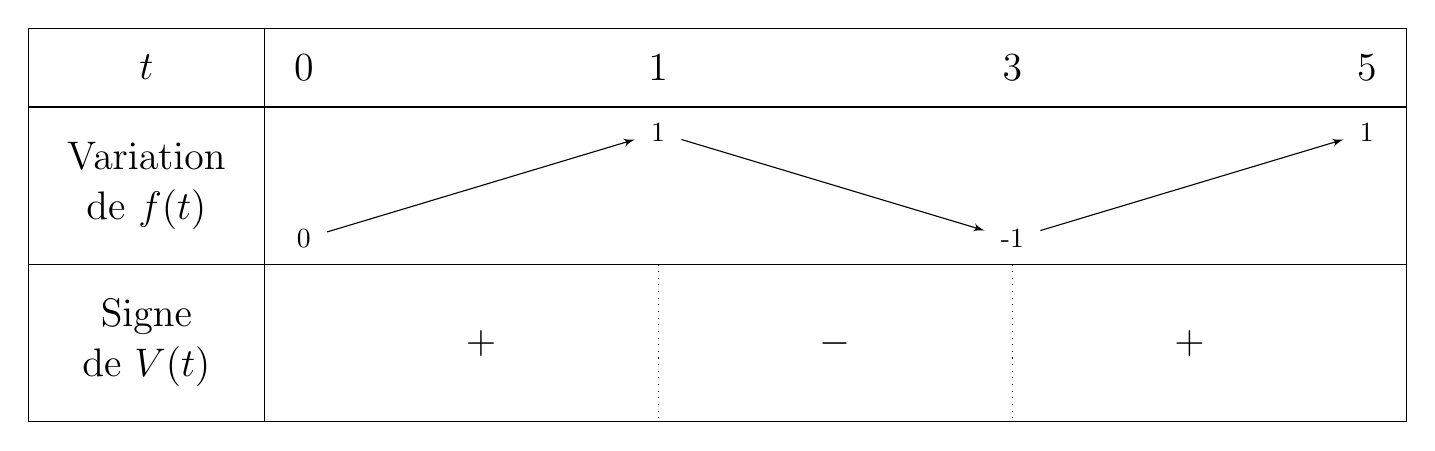
\begin{tikzpicture}
		\tkzTabInit
		 %[lgt=3,espcl=1.5]
		 [lgt=3,espcl=4.5]
	       		{$t$ / 1 , Variation de $f(t)$ / 2, Signe de $V(t)$ / 2}
	       		{0,1,3,5}
		\tkzTabVar
			{-/0,+/1,-/-1,+/1}
			
		\tkzTabLine
			{,+,t,-,t,+}
	\end{tikzpicture}
	
	% page 3-6
	\begin{tikzpicture}
	\begin{axis}[xmin = 0, xmax=5, ymin=-1.25, ymax=1.25, grid = none,  xlabel={$t$}, ylabel={$f(t)$}]
		\addplot[domain=0:5, samples=500, BLUE_E, thick] {sin(90*x)};
		\addplot[<->, domain=3.2:4.8, samples=2, RED_E, thick] {x-4};
	\end{axis}
	\end{tikzpicture}
	\begin{tikzpicture}
	\begin{axis}[xmin = 0, xmax=5, ymin=-1.25, ymax=1.25, grid = none,  xlabel={$t$}, ylabel={$f(t)$}]
		\addplot[domain=0:5, samples=500, BLUE_E, thick] {sin(90*x)};
		\addplot[<->, domain=3.2:4.8, samples=2, RED_E, thick] {.9876/.9*(x-4)};
	\end{axis}
	\end{tikzpicture}
	\begin{tikzpicture}
	\begin{axis}[xmin = 0, xmax=5, ymin=-1.25, ymax=1.25, grid = none,  xlabel={$t$}, ylabel={$f(t)$}]
		\addplot[domain=0:5, samples=500, BLUE_E, thick] {sin(90*x)};
		\addplot[<->, domain=3.2:4.8, samples=2, RED_E, thick] {.95105/.8*(x-4)};
	\end{axis}
	\end{tikzpicture}
	\begin{tikzpicture}
	\begin{axis}[xmin = 0, xmax=5, ymin=-1.25, ymax=1.25, grid = none,  xlabel={$t$}, ylabel={$f(t)$}]
		\addplot[domain=0:5, samples=500, BLUE_E, thick] {sin(90*x)};
		\addplot[<->, domain=3.2:4.8, samples=2, RED_E, thick] {.89100/.7*(x-4)};
	\end{axis}
	\end{tikzpicture}
	
	% page 7
	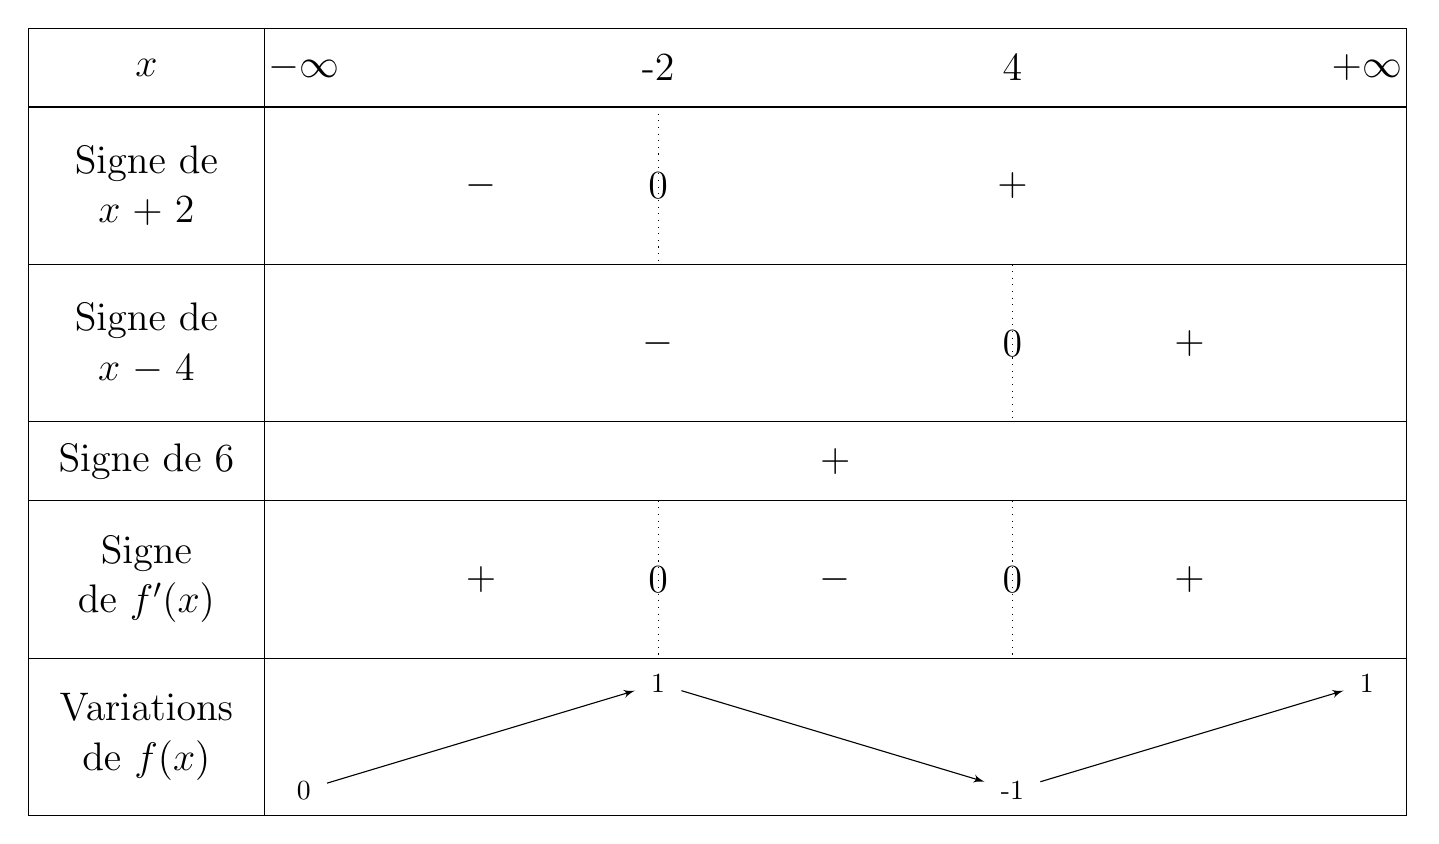
\begin{tikzpicture}
		\tkzTabInit
		 %[lgt=3,espcl=1.5]
		 [lgt=3,espcl=4.5]
	       		{$x$ / 1 , Signe de $x+2$ / 2, Signe de $x-4$ / 2, Signe de $6$ / 1, Signe de $f'(x)$ / 2, Variations de $f(x)$ / 2}
	       		{$\minfty$, -2, 4, $\pinfty$}
			
		\tkzTabLine
			{,-,z,,+,}
		\tkzTabLine
			{,,-,,z,+}
		\tkzTabLine
			{,,,+,,}
		\tkzTabLine
			{,+,z,-,z,+}
			
		\tkzTabVar
			{-/0,+/1,-/-1,+/1}
	\end{tikzpicture}
%
\end{document}